\documentclass[twosided,a4paper]{article}           %type
\usepackage[top=2cm,bottom=2cm,inner=1.5cm,outer=1.5cm]{geometry}       %geometry
\renewcommand{\familydefault}{\sfdefault}
\usepackage[sfdefault, light]{roboto}

%\usepackage[italian]{babel}                %font/language
\usepackage[T1]{fontenc}
\usepackage[utf8]{inputenc}

\usepackage{amsmath}                       %maths
\usepackage{bm}
\usepackage{amssymb}					   %for numbersets

\usepackage{graphicx}
\usepackage{epstopdf} 
\usepackage{float}
\usepackage{subfigure}

\usepackage{tabularx}
\usepackage{multirow}

%  EXOTIC STUFF %%%%%%%%%%%%%%%%%%%%%%%%%%%%%%%%%%%%%%%%%%%%%%%%%%
\newcommand*{\TakeFourierOrnament}[1]{{%                         %
		\fontencoding{U}\fontfamily{futs}\selectfont\char#1}}    %
\newcommand*{\danger}{\TakeFourierOrnament{66}}                  %          
                                                                 %
\usepackage{newunicodechar}

\newcommand\Warning{%
	\makebox[1.4em][c]{%
		\makebox[0pt][c]{\raisebox{.1em}{\small!}}%
		\makebox[0pt][c]{\color{red}\Large$\bigtriangleup$}}}

\newunicodechar{⚠}{\Warning}
%%%%%%%%%%%%%%%%%%%%%%%%%%%%%%%%%%%%%%%%%%%%%%%%%%%%%%%%%%%%%%%%%%

%rapid file input
\newcommand{\rs}[1]{\input{result/#1.txt}}

%create new environment with enumeration
                    
\newcounter{comment}[section]
\newenvironment{comment}[1][]{\refstepcounter{comment}\par\medskip
	\noindent \textbf{Comment~\thecomment. #1} }{\par}

\newcounter{box}
\newenvironment{scatola}[1]
{\refstepcounter{box}
\begin{center}
		\begin{tabular}{|p{\linewidth}|}
			\hline \textbf{Box~\thebox} #1  \\
		}
		{ 
			 \\ \hline
		\end{tabular} 
	\end{center}
 }


%\usepackage{hyperref}

%\usepackage{subfloat}
%full packaging for image in eps finally
\usepackage{textcomp}

\usepackage{color}
\usepackage[dvipsnames]{xcolor}

\usepackage{listings} 

\newcommand{\tr}{^{{\bm \top}}}

\newenvironment{sistema}%
{\left\lbrace\begin{array}{@{}l@{}}}%
	{\end{array}\right.}

\begin{document}
	
	\title{\textcolor{MidnightBlue}{Mechanical vibration} - \textcolor{Plum}{System identification and modal analysis of 3-DOF linear system}}
	\author{Giammarco Valenti}
	\maketitle
	
\section{Dynamical system}
\subsection{The system and the experimental setup}
The system consists of three different bodies on three carriers. The carriers are aligned and the bodies are constrained to slide along the common axis. Between the bodies two springs are located, and a third spring connects the frame and the last body. The first body is rigidly connected trough a rack-pinion gearing with a motor which is controlled in voltage with a PC interface. The position of each body is provided by an encoder. The zeroes of the positions are at the springs rest position. The scheme of the model is depicted in Figure \ref{fig:theplant1}.
The displacement of the masses in meters is available from the encoder with the following resolution:
\begin{equation}
	\Delta x = \dfrac{2 \pi r_e}{16000}.
	\label{eq:enc_res}
\end{equation}
\subsection{The dynamical model}
\subsubsection{Assumptions}
\label{sec:ass}
To define a model of the system, some assumptions were made:
\begin{description}
	\item[Rectilinear motion] All the bodies (masses), and the rack of the rack-pinion gearing are supposed to move and exert forces along the same axis, which is the motion axis. Consequently, all the quantities are meant to be projected on this axis.
	\item[Viscous friction] Only viscous frictions are present
	\item[Instantaneous electrical dynamics] The model of the electrical dynamics of the motor is only a gain from voltage to force, expressed by the voltage-to-force factor, which is exploited in Section \ref{sec:step}.
	\item [Motor mechanics merged] Inertia and damping of the motor are merged respectively into $m_1$ and $c_1$ (refer to Figure \ref{fig:theplant1})
	\begin{equation}
	\begin{sistema}
	m_1 = m_{block} + \frac{J_{motor}\vert_{zz}}{r^2}\\
	c_2 = c_{block} + \frac{c_{motor}}{r^2}
	\end{sistema}
	\end{equation}
	where $r$ is the radius of the gear-rack coupling (gear wheel), $J_{motor}\vert_{zz}$ is the inertia of the motor , $c_{motor}$ the rotational damping and ''block'' quantities are the ones stricly related to the physical first mass.
	\item [Last viscosities merged] The term $c_3$ (refer to Figure \ref{fig:theplant1}) contains the viscous friction with the ground and the one due to the spring. In the model those two contributions cannot be quantified separately.
\end{description}
\subsubsection{The linear model}
\label{sec:linear_sys}



The chosen model is a linear plant consisting of 3 lumped masses, 3 lumped springs between them (the last to the frame), and 3 dampers between each mass and the ground. The model is shown in Figure \ref{fig:theplant1}.
\begin{figure}[H]
	\centering
	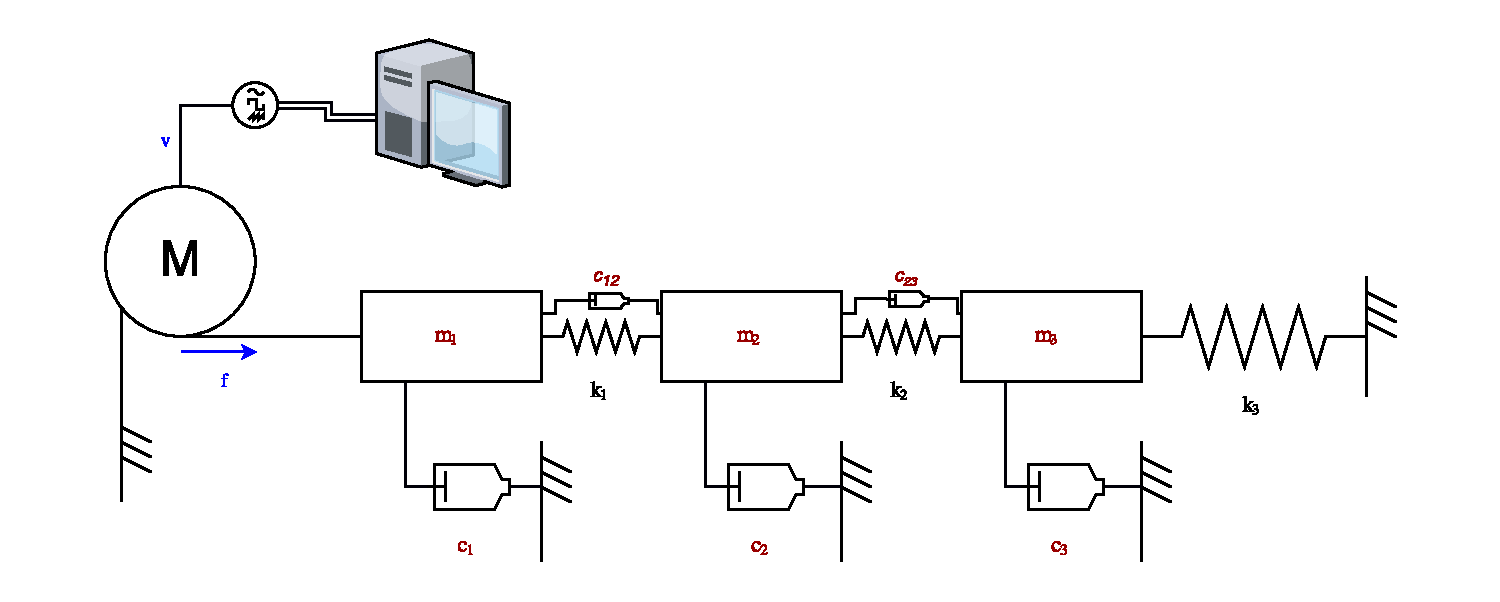
\includegraphics[width=\linewidth]{img/theplant1}
	\caption[The linear plant]{The chosen plant, in red the unknown parameters}
	\label{fig:theplant1}
\end{figure} %TODO figure with displacements x
\subsection{equation of motion}
\begin{equation}
	\begin{sistema}
	m_1 \ddot{x}_1 = + k_1 \left (x_2 - x_1 \right )                                 + c_{12} \left ( \dot{x}_2 - \dot{x}_1 \right )                                                  - c_1\dot{x}_1 + g_v v(t)\\
	m_2 \ddot{x}_2 = + k_1 \left (x_1 - x_2 \right ) + k_2 \left (x_3 - x_2 \right ) + c_{12} \left ( \dot{x}_1 - \dot{x}_2 \right ) +  c_{23} \left ( \dot{x}_3 - \dot{x}_2 \right ) - c_2\dot{x}_2\\
	m_3 \ddot{x}_3 =                                 + k_2 \left (x_2 - x_3 \right )                                                 +  c_{23} \left ( \dot{x}_2 - \dot{x}_3 \right ) - c_3\dot{x}_3 - k_3 x_3
	\end{sistema}
\end{equation}
In the classical matrix form:
\begin{subequations}
\begin{equation}
	\bm M \ddot{x} + \bm C \dot{x} + \bm K x = \bm b
	\label{eq:eqm:tot}
\end{equation}
where:\\
	\begin{tabularx}{\linewidth}{@{}XXX@{}}
	\begin{equation}
\bm K = \left[ \begin{array}{ccc}
+ k_1  & - k_1 & 0 \\ 
-k_1 & + k_1 + k_2 & -k_2 \\ 
0 & - k_2 & + k_3
\end{array}  \right]
\label{eq:eqm:K}
\end{equation} &
	\begin{equation}	
		\bm M = \left [\begin{array}{ccc}
		m_1 & 0 & 0 \\ 
		0 & m_2 & 0 \\ 
		0 & 0 & m_3
	\end{array} \right ]
	\label{eq:eqm:M}
\end{equation} \\
	\begin{equation}
\bm b = \left[ \begin{array}{ccc}
g_v \\ 0 \\  0
\end{array}  \right]
\label{eq:eqm:b}
\end{equation} &
	\begin{equation}
	\bm C = \left[\begin{array}{ccc}
	+ c_1 + c_{12} & -c_{12} &  0 \\ 
	-c_{12} & +c_2 + c_{12} + c_{23} & -c_{23} \\ 
	0 & -c_{23} & c_3 + c_{23} 
	\end{array} \right]
	\label{eq:eqm:C}
	\end{equation}
	\end{tabularx}
\label{eq:Mtot}
\end{subequations}
\subsection{state-space model}
	The linear model of the plant, expressed by the equation \eqref{eq:Mtot}, is a SIMO model. A state-space form was chosen to represent this model. The matrices are the follwing:\\
\begin{subequations}
\begin{tabularx}{\linewidth}{@{}XXX@{}}
	\begin{equation}
	\begin{sistema}
		\dot{x} = \bm{A}x + \bm{B}v\\
		      y = \bm{C}x + \bm{D}v
	\end{sistema}
	\end{equation}&
	\begin{equation}
		x = \left [ \begin{array}{cccccc}
		x_1 & x_2 & x_3 & \dot{x}_1  & \dot{x}_2 & \dot{x}_3 
		\end{array}  \right ]\tr
	\end{equation}\\
	\begin{equation}
		A = \left [ \begin{array}{cc}
		\bm Z_{3 \times 3} & \bm I_{3 \times 3} \\ 
		\bm{-M^{-1}K} & \bm{-M^{-1}C}
		\end{array} \right ]
		\label{eq:ss:A}
	\end{equation} &
	\begin{equation}
	\bm B =	\left [ \begin{array}{c}
		\bm Z_{3\times 1} \\ 
		\bm{-M^{-1}b}
		\end{array} \right ]
		\label{eq:ss:B}
	\end{equation} \\
		\begin{equation}
	\bm C =	\left [\begin{array}{cc}
	\bm I_{3\times 3} & \bm Z_{3\times 3}
	\end{array}   \right ]
	\label{eq:ss:C}
	\end{equation} &
	\begin{equation}
	\bm D =	\left [\begin{array}{c}
	\bm Z_{3 \times 1}
	\end{array}   \right ]
	\label{eq:ss:D}
	\end{equation} 
\end{tabularx}
\label{eq:ss}
\end{subequations}
where $\bm I$ is the identity matrix and $\bm Z$ is a matrix with all the entries equal to zero.
\subsection{experimental setup}
\subsubsection{data processing}
Few operations on data must be performed in order to use them. At first, the data on diplacements is provided in \textit{encoder counts}. They are converted in meters with the following convertion factor ($g_x$):
\begin{equation}
	g_x = \dfrac{\Delta x}{\Delta \texttt{counts}} = 2 \pi r_e \cdot \dfrac{\Delta \texttt{counts}}{16000\dfrac{\texttt{counts}}{\texttt{encoder revolution}}}.
\end{equation}
	\subsection{parameters and data available}
The linear system in Section \ref{sec:linear_sys} is fully represented by parameters, they are shown in Table \ref{tab:parameters}. Only the stiffnesses of the springs ($k_i$) are known.
\begin{table}[H]
	\centering
	\label{tab:parameters}
	\begin{tabular}{|l||l||l|l|l||l|l|l||l|l|l|l|l||}
		\hline
		Name & $g_v$ & $k_1$ & $k_2$ & $k_3$ &  $m_1$ & $m_2$ & $m_3$  &  $c_1$ & $c_2$ & $c_3$  & $c_{12}$ & $c_{23}$ \\
		\hline
		Value & - & \input{result/k1.txt} & \input{result/k2.txt} & \input{result/k3.txt} & - & - & - & - & - & - & - & - \\ 
		\hline
		Units& N/V & \multicolumn{3}{l||}{$N/m$} & \multicolumn{3}{l||}{$K_g$} & \multicolumn{5}{l||}{$Ns \ m^{-1}$} \\ \hline
		Notes &       &       &       &       &       &    &   & \multicolumn{5}{l||}{\small{$c_a$ and $c_b$ if proportional damping}} \\ \hline
	\end{tabular}
\caption{Parameters  ( ''-'' stands for unavailable parameter)}
\end{table}
The meaning of each parameter is depicted in Figure \ref{fig:theplant1}, except for the  \textit{voltage-to-force} coefficient. Such coefficient $g_v$ is the factor which converts the voltage of the signal sent to the motor in the force exerted on the rack. It is the product of several physical gains as shown in Equation \eqref{eq:g_v}.
\begin{equation}
f = (k_a\cdot k_t \cdot k_{mp})v(t) = g_v v(t).
\label{eq:g_v}
\end{equation}
Where the physical meanings are:\\
\begin{subequations}
	\begin{tabularx}{\linewidth}{ X | X | X }
		\centering
		\begin{equation}
			k_a = \dfrac{1}{R_{motor}} \approx 2 \ AV^{-1}
		\end{equation} Electrical conductance of the motor &
		\centering
		\begin{equation}
			k_t \approx 0.1 \ NmA^{-1}
		\end{equation} Motor torque constant&
		\centering
		\begin{equation}
			k_{mp} = \dfrac{1}{r_{pinion}} \approx 26.25 \  m^{-1}
		\end{equation} Trasmission ratio of the gearing
	\end{tabularx}
\end{subequations}

\section{System identification}
	
\subsection{steady state analysis}
\label{sec:step}
From the \textit{step response analysis} the steady state values of input and output are considered. In this analysis the ''static'' coefficients can be studied, they are:
\begin{itemize}
	\item voltage to force $g_v$
	\item springs' stiffness $k_i$ with $i \in 1,2,3$
\end{itemize} 
The goal of this section is to estimate $g_v$ and to verify the ratios between the stiffnesses $k_i$, w.r.t the nomina values. It is not possible to verify directly the $k_i$ values because the steady state values are $3$ as many as the equations of the generated system (linear) while the variables would be $4$.
\subsubsection{Calculations}
In order to generate the system of equations, the static gain vector $g_{dc}$ of the system is computed. A procedure may be to apply the ''CAB'' formula from the state space formulation:
\begin{equation}
\label{eq:cab}
	\bm{g_{dc}} =	\bm{CA^{-1}B}.
\end{equation}
which is the transfer function at $s = 0$. Since equation \eqref{eq:cab} implies the inverse of the $6 \times 6$ matrix $\bm A$, another computation is performed. Using the formulation in Equation \eqref{eq:Mtot}, the following limits are performed:
\begin{equation}
	\begin{sistema}
	\lim_{t \to + \infty}{\dot{x}}  = 0  \\
	\lim_{t \to + \infty}{\ddot{x}} = 0
	\end{sistema}
	\label{eq:dot_limits}
\end{equation}
The substitution \eqref{eq:dot_limits} in \eqref{eq:eqm:tot} yields:
\begin{equation}
\bm K x = \bm b
\label{eq:dot0}
\end{equation} The static gain is then:
\begin{equation}
	\bm{g_{dc}} = \bm{K^{-1}}\bm{b}
\end{equation}


\begin{equation}
	\bm{g_{dc}} =
	\left [ \begin{array}{ccc}
	g_v\dfrac{k_1k_2 + k_3k_2 + k_3k_1}{k_1k_2k_3}  & g_v\dfrac{k_2+k_3}{k_2k_3} & g_v\dfrac{1}{k_3}
	\end{array} \right ]\tr
	\label{eq:g_dc}
\end{equation}
\begin{comment}
Apply \eqref{eq:dot_limits} to equation \eqref{eq:eqm:tot} is equivalent to apply the Laplace tranform to the equation
\eqref{eq:eqm:tot} and apply the final value theorem to it
\end{comment}
\begin{comment}
Looking at the Equation \eqref{eq:g_dc} is evident the series connection of the springs.
\end{comment}\vspace{0.2 cm}
\noindent The steady state value of the three output are available. Some other computations has to be made to make equation \eqref{eq:g_dc} suitable for the check on the stiffnesses ratios and the new estimation of $g_v$. The equation for the steady state values is:
\begin{equation}
	\bm{C}\bm{x}_\infty = \bm{g_{dc}}v_\infty  
	\label{eq:stst1}
\end{equation}
Where the $\infty$ denotes the steady state value of the quantity ($\lim_{t \to \infty}{f(t)}$). The Equation \eqref{eq:stst1} is now expressed in terms of stiffnesses ratio: $k_3$ is fixed to the nominal value and two ratio are defined as following.\\
\begin{subequations}
	\centering
	\begin{tabularx}{\linewidth}{X X}
		\begin{equation}
			R_{31} = \dfrac{k_3}{k_1}
		\end{equation} &
		\begin{equation}
			R_{32} = \dfrac{k_3}{k_2}
		\end{equation}
	\end{tabularx}
\end{subequations}
This operations are made in order to make the system easy to solve, and uncoupling the nonlinear factor $g_v$. This allows to solve the system in a cascade fashion from $g_v$ to $R_{13}$. The equation \eqref{eq:stst1} is now expressed in the following form:
\begin{equation}
	\label{eq:stst2} 
	k_3 \left [\begin{array}{c}
	x_1(\infty) \\ 
	x_2(\infty) \\ 
	x_3(\infty) \end{array}  \right ] 
	=
	u(\infty)\left [\begin{array}{c}
	g_v + g_v R_{13} + g_v R_{23} \\ 
	g_v R_{23} \\ 
	g_v \end{array}  \right ] 
\end{equation}
\subsubsection{Steady state value picking}
Now the next step is to use the measured value of steady state response (input and output), take $g_v$ as new estimated value and verify that $R_{12}$ and $R_{32}$ matches the nominal values. The input is set on $u(\infty) = 0.5$.\\
The value of steady state response are picked from the data directly, as shown in Figure \ref{fig:stst1}. The input is shown in Figure \ref{fig:step_input}.
\begin{figure}[H]
	\centering
	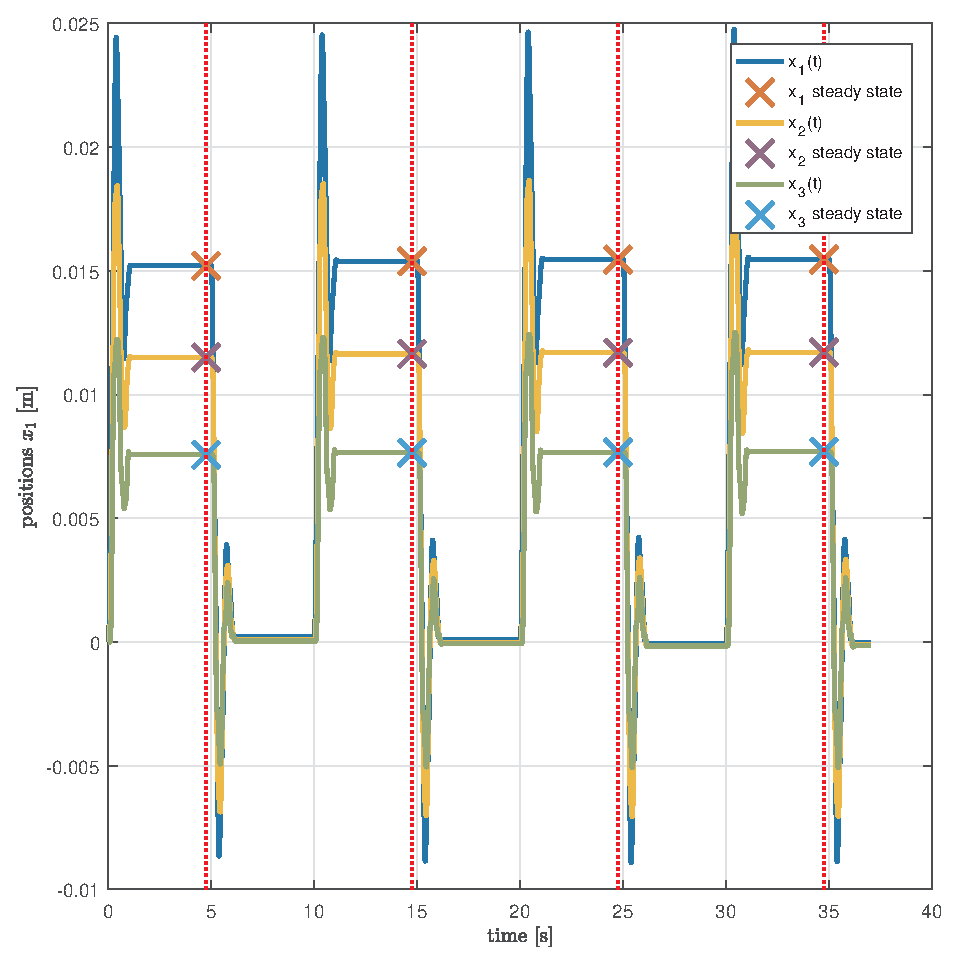
\includegraphics[width=\linewidth]{img/stst1}
	\caption[steady state value picking]{Steady state value picking}
	\label{fig:stst1}
\end{figure}
\begin{figure}[H]
	\centering
	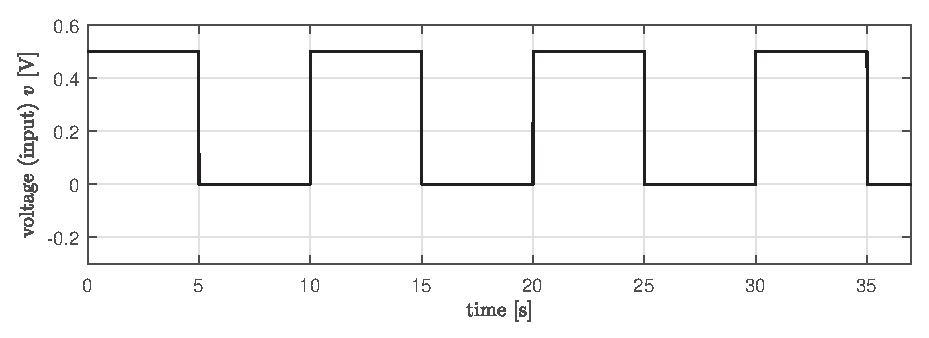
\includegraphics[width=\linewidth]{img/step_input}
	\caption{Step input}
	\label{fig:step_input}
\end{figure}
\noindent
The obtained values for each output ($\bm x_{\infty}$) are $4$. The mean value of the ratios ($R31$,$R32$) is estimated by the \textbf{arithmetic average}. Given ($ \bm x_{\infty}$) averaged from the data, Equation \eqref{eq:stst2} is solved and the results are shown in Table \ref{tab:ratios}. The error is defined as $\texttt{error}\% = 100\dfrac{data \ value}{nominal}$
%TODO< write the mambo jambo
\begin{table}[H]
	\centering
	\begin{tabular}{|c|c|c|c|}
		\hline 
		 & from data & nominal & error \% \\ 
		\hline 
		$k_3/k_2$ & \input{result/R32_exp.txt}& \input{result/R32_nom.txt} & \input{result/R32_per.txt}\%  \\ 
		\hline 
		$k_3/k_1$ & \input{result/R31_exp.txt}& \input{result/R31_nom.txt} & \input{result/R31_per.txt}\% \\
		\hline \hline
		      & from data              & initial & error 
		      \%\\
		\hline
		$g_v$ & \input{result/g_v.txt} & \input{result/gain_v.txt} & \input{result/g_v_per.txt}\% \\\hline
	\end{tabular} 
	\label{tab:ratios}
	\caption{Stiffnesses ratios and voltage-to-force coefficients results from steady state analysis}
\end{table}
The \textit{voltage-to-force} estimation is shown in table \ref{tab:ratios}.
\subsection{Parameters estimation}
To estimate the parameters the impulse response is used. The \textit{voltage-to-force} coefficient $g_v$ is one of the parameters to be estimate in order to include the possibility to cross-check the result with the step response result.
The parameters to estimate are shown in table \ref{tab:parameters}.
\subsubsection{Estimation strategy}
	\label{sec:est_strat}
 The strategy to estimate the parameters consists in use the \textbf{linear model} described in \ref{sec:linear_sys}, use the same input as the real model, and compare the output with the real output tuning the parameters to minimize the difference.
\begin{scatola}{Estimation strategy keypoints}
	\label{box:est_stra}
 \begin{enumerate}
	 \item Choose the linear model
	 \item Provide the same input as the real system (an impulse-like signal)
	 \item Simulate the output (time domain)
	 \item Compare the outputs with the real one.
	 \item Computing the sum of squares of the residuals
	 \item Tune the parameters iterativly to minimize this quantity
 \end{enumerate}
\end{scatola}
The implementation of the strategy in Box \ref{box:est_stra} is possible creating a MATLAB function which presents in input the parameters and in output the sum of the squares of the residuals. This is performed with a simulation of the system executed inside the function, the data of the real system are available as a global variable, and the only output is the sum of square to minimize. The strategy and the function to minimize (orange box) is shown in Figure \ref{fig:eststrategy}.
\begin{figure}[H]
	\centering
	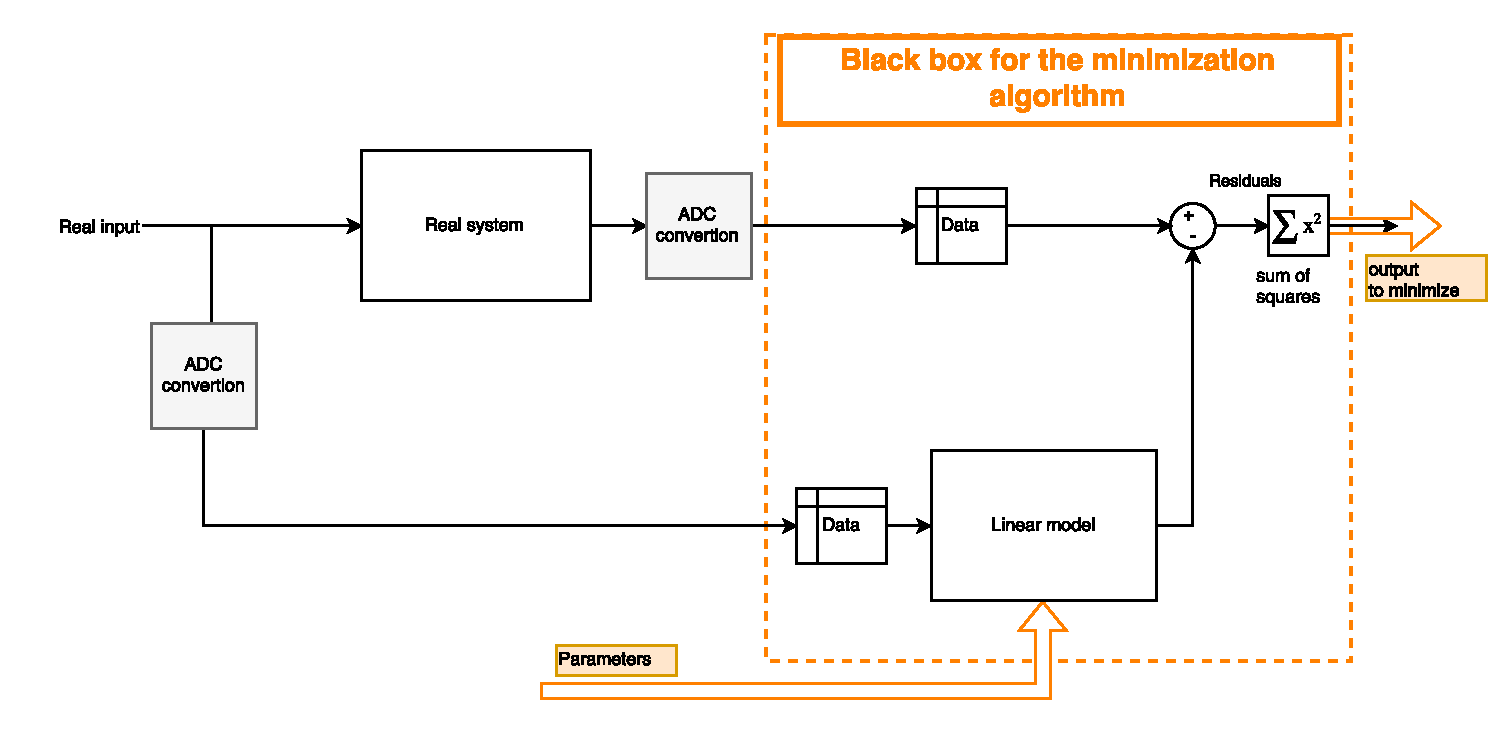
\includegraphics[width=\linewidth]{img/est_strategy}
	\caption{estimation strategy scheme, Function to minimize in \textcolor{orange}{orange}}
	\label{fig:eststrategy}
\end{figure}
\begin{comment}
	A single evaluation of the function corresponds to a simulation of the linear system, the parameters are updated by the algorithm after the evaluation of the function\\
\end{comment}
\noindent The implementaion of the strategy is performed with MATLAB, the function \texttt{\textbf{lsqnonlin}} is used. The input used is a pulse-like waveform which excite the system four times, the 
signal is shown in Figure \ref{fig:pulse_input}.
\begin{figure}
	\centering
	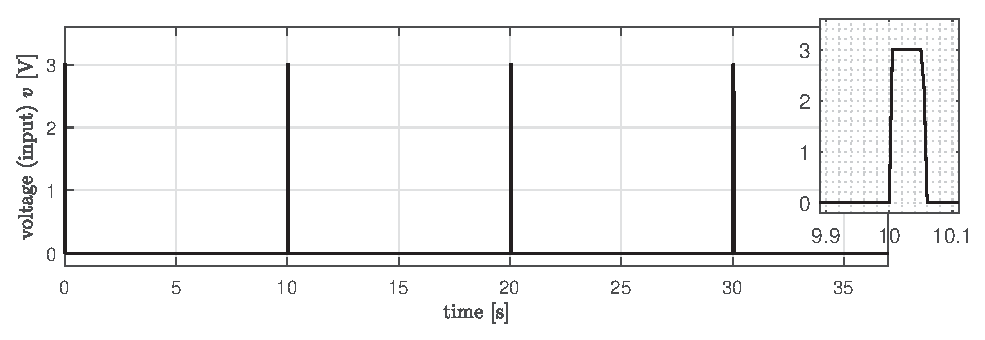
\includegraphics[width=\linewidth]{img/pulse_input}
	\caption{The pulse-like input (zoom of the single pulse on the right)}
	\label{fig:pulse_input}
\end{figure}


\subsubsection{Free damping case}
The first estimation is performed using the model in Equations \eqref{eq:ss}.

%TODO first guesses

The results of this optimization are shown in table \ref{tab:est_full_results}
\begin{table}[H]
	\centering
	\label{tab:est_full_results}
	\begin{tabular}{|l|l|l|l|l|l|l|l|l|l|}
		\hline
		Name & $g_v$ &  $m_1$ & $m_2$ & $m_3$  &  $c_1$ & $c_2$ & $c_3$  & $c_{12}$ & $c_{23}$ \\
		\hline
		Value & \input{result/g_v_est_f.txt} & \input{result/m1_f.txt} & \input{result/m2_f.txt} & \input{result/m3_f.txt} & \input{result/c1_f.txt} & \input{result/c2_f.txt} & \input{result/c3_f.txt} & \input{result/c12_f.txt} & \input{result/c23_f.txt} \\ 
		\hline
		Unit & $N/V$ &  \multicolumn{3}{l|}{$K_g$}  &  \multicolumn{5}{l|}{$Ns \ m_{-1}$} \\
		\hline
\end{tabular}
\caption{Estimation results (model with free damping)}
\end{table}
A plot with the comparison of the models is provided in Figure \ref{fig:compare_f}. The normalized root means square errors are provided for each DOF in table \ref{tab:fit_all}
\begin{figure}[H]
	\centering
		\caption{Comparison between the response of the model and the response of the system}
	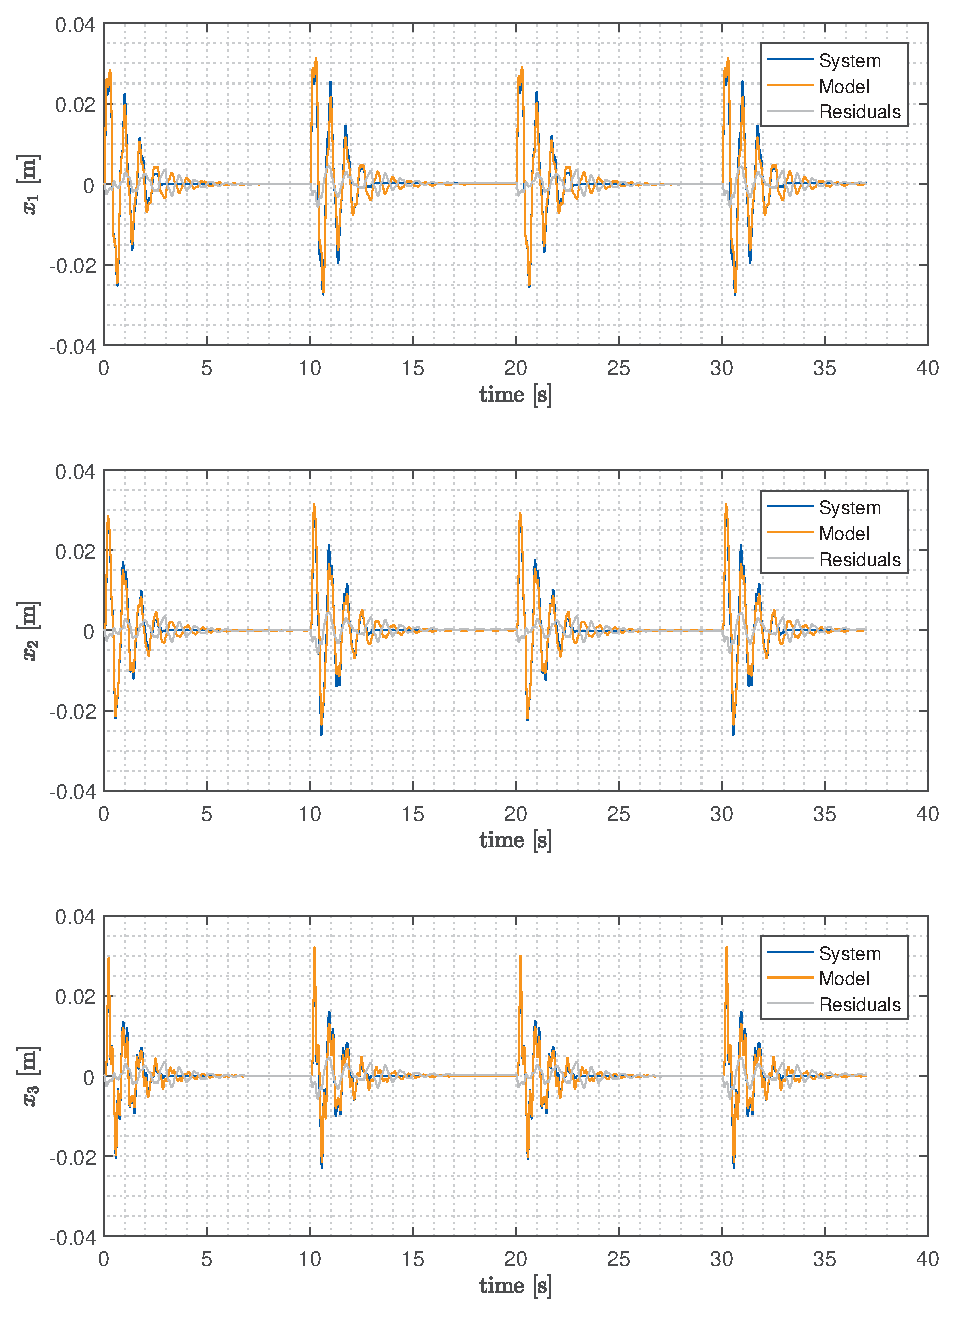
\includegraphics[width=\linewidth]{img/compare_f}
	\label{fig:compare_f}
\end{figure}
\subsubsection{Proportional damping case}
The procedure is exactly the same as the case of the free damping. The parameters to estimate now are 6 instead of 9. The damping now is represented by only 2 parameters, as shown in Equation \eqref{eq:prop_C}.
\begin{equation}
	\label{eq:prop_C}
	\bm{C} = c_a\bm{M} + c_b\bm{K}
\end{equation}
\begin{table}[H]
	\centering
	\label{tab:est_prop_results}
	\begin{tabular}{|l|l|l|l|l|l|l|l|l|l|}
		\hline
		Name & $g_v$ &  $m_1$ & $m_2$ & $m_3$  &  $c_a$ & $c_b$  \\
		\hline
		Value & \input{result/g_v_est_f.txt} & \input{result/m1_f.txt} & \input{result/m2_f.txt} & \input{result/m3_f.txt} & \input{result/ca_p.txt} & \input{result/cb_p.txt} \\ 
		\hline
		Unit & $N/V$ &  \multicolumn{3}{l|}{$K_g$}  &  \multicolumn{2}{l|}{$Ns \ m_{-1}$} \\
		\hline
	\end{tabular}
	\caption{Estimation results (model with proportional damping)}
\end{table}
\begin{figure}[H]
	\centering
	\caption{Comparison between the response of the model and the response of the system - proportional damping case}
	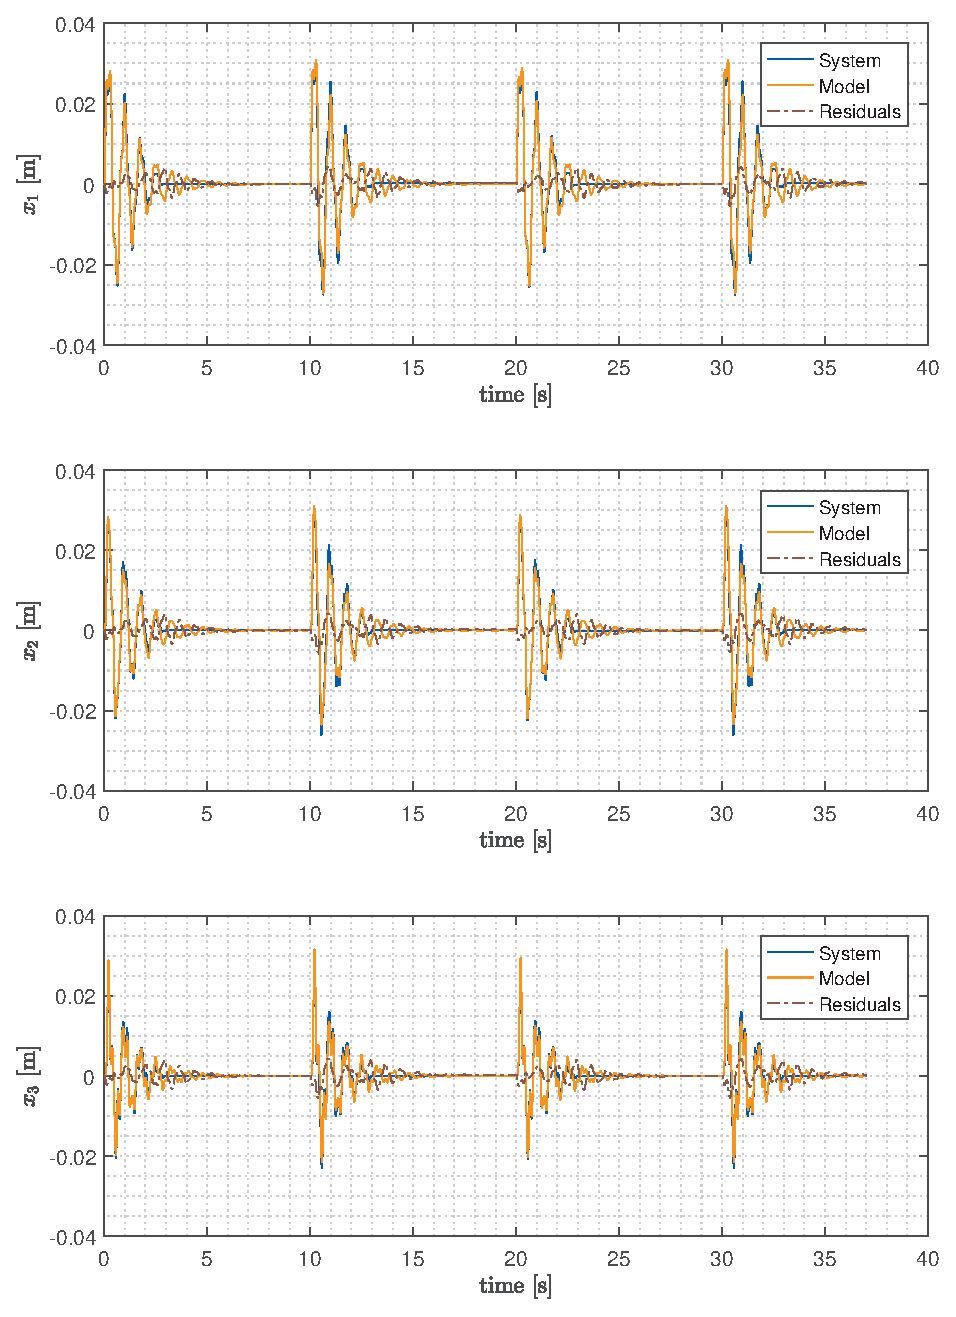
\includegraphics[width=\linewidth]{img/compare_p}
	\label{fig:compare_p}
\end{figure}
%TODO friction
%TODO statistics
%TODO good estimation non liner stuff 20% (friction)

\begin{table}[]
	\centering
	\caption{NRMSE for the outputs}
	\label{tab:fit_all}
	\begin{tabular}{l|l|l|}
		\cline{2-3}
		& Free damping  & Proportional damping \\ \hline
		\multicolumn{1}{|l|}{$x_1$ \texttt{NRMSE} } & \input{result/fit_f1.txt} \%        &         \input{result/fit_p1.txt} \%             \\ \hline
		\multicolumn{1}{|l|}{$x_2$ \texttt{NRMSE} } &  \input{result/fit_f2.txt} \%             &       \input{result/fit_p2.txt} \%           \\ \hline
		\multicolumn{1}{|l|}{$x_3$ \texttt{NRMSE} } &   \input{result/fit_f3.txt} \%  &
		\input{result/fit_p3.txt} \%                              \\ \hline
	\end{tabular}
\end{table}
\section{modal analysis}
\subsection{Eigenvalue problem}
\label{sec:eigenvalueproblem}
Define a system expressed by the following equation:
\begin{equation}
\bm M \ddot{x}(t) + \bm K x(t) = \bm bv(t)
\label{eq:eqm:und}
\end{equation} 
this system is the \textbf{undamped} version of system \eqref{eq:Mtot}.
The natural frequencies of the system in Equation \eqref{eq:Mtot} (the same as equation \ref{eq:eqm:und}) can be derived solving an eigenvalue problem stated as follows:
\begin{scatola}{The natural frequencies , modal shape vectors and eigenvalue problem}
	\label{box:eig_prob}
	 \\
			Given the system expressed in \eqref{eq:Mtot} define a natural frequency an $\omega > 0$ with $x_e \neq 0_v \in \Re^3 $ such that :
		\begin{equation}
		\label{eq:eigenproblem}
			\left( \bm{K} -\omega^{2}\bm{M} \right )x = 0_v 
		\end{equation}
		Equation \eqref{eq:eigenproblem} is equivalent to Equation \eqref{eq:ker_det}.
		\begin{equation}
		\label{eq:ker_det}
			Ker\left( \bm{K} -\omega^{2}\bm{M} \right ) \neq 0_v \quad \Leftrightarrow  \quad det\left( \bm{K} -\omega^{2}\bm{M} \right ) = 0
		\end{equation}
	The quantities $\omega$ are the \textbf{natural frequencies} of the system, and the eigenvectors $x_e$ are the \textbf{modal shape vectors} of the system. Associate a frequency $\omega$ with its square $\omega^2$ which is an eigenvalue of \eqref{eq:eigenproblem}, take the corresponding eigenvector and define the pairs:
	\begin{equation}
		(u_i,\omega_i) \quad i \in \left \lbrace 1,2,3\right \rbrace
	\end{equation}
	Define the \textbf{Modal shape matrix}, the matrix of column vector $u_i$ sorted by increasing frequency.
	\begin{equation}
		\bm{U} = \left [\begin{array}{ccc}
		u_1 & u_2 & u_3
		\end{array} \right ]
	\end{equation}
\end{scatola}
\begin{comment}
solving the problem in the Box \ref{box:eig_prob}, is equivalent to find the poles of the transfer function between the input and the output of the undamped system \ref{eq:eqm:und}. the poles are $\pm i\omega$.\\
\end{comment}
To solve proble in Box \ref{box:eig_prob} MATLAB provides a function \texttt{eig}, which receives in input the two matrices ($\bm{K}$ and $\bm{M}$) and returns the eigenvalues and the eigenvectors in a matrix. Taking the square root of the ladders the $\omega$ are obtained, the Modal shape matrix is directly provided by the function.
The modal shape vectors are orthogonal each other and this is a property which can be verified.
\subsubsection{Results}
The procedure shown in the previous Section \ref{sec:eigenvalueproblem} is the same for both the case of Free damping and proportional damping. The difference leads in the different value estimated. They are shown in table \ref{tab:est_full_results} and \ref{tab:est_prop_results}.
The value obtained from the eigenvalue problem are shown in table \ref{tab:eig_results}.


% Please add the following required packages to your document preamble:
% \usepackage{multirow}
\begin{table}[H]
	\centering
	\caption{Values of frequencies and modal shapes vector obtain solving the eigenvalue problem}
	\label{tab:eig_results}
	\begin{tabular}{|l|lll|lll|}
		\hline
		& \multicolumn{3}{l|}{Free damping}                                                           & \multicolumn{3}{l|}{proportional damping}                                                   \\ \hline
		$\omega$  [rad/s]               & \multicolumn{1}{l|}{\rs{w_f_1}} & \multicolumn{1}{l|}{\rs{w_f_2}} & \rs{w_f_3}  & \multicolumn{1}{l|}{\rs{w_p_1}} & \multicolumn{1}{l|}{\rs{w_p_2}} & \rs{w_p_3}  \\ \hline
		\multirow{3}{*}{$\bm U$} & \rs{U_f_11}                     & \rs{U_f_12}                     & \rs{U_f_13} & \rs{U_p_11}                     & \rs{U_p_12}                     & \rs{U_p_13} \\
		& \rs{U_f_21}                     & \rs{U_f_22}                     & \rs{U_f_23} & \rs{U_p_21}                     & \rs{U_p_22}                     & \rs{U_p_23} \\
		& \rs{U_f_31}                     & \rs{U_f_32}                     & \rs{U_f_33} & \rs{U_p_31}                     & \rs{U_p_32}                     & \rs{U_p_33} \\ \hline
	\end{tabular}
\end{table}















\subsection{Raileight method}
The Raileight method is a method to find simultaneously the natural frequencies and the modal shapes vector. Ths method is based on the search of stationary point in a function, the Raileight quotient.
The Rayleight quotient is 
	\begin{equation}
		R_q(\bm x) = \dfrac{\bm x\tr \bm K \bm x}{\bm x\tr \bm M \bm x} .
	\end{equation}
The Raileight quotient manifests two properties which make it suitable to do so:
\begin{enumerate}
	\item Given an eigenvector (modal shape vector) $R_q(U_i)$ = $\omega_i^2$
	\item $R_q(x)$ Presents a stationary point in the neighborhood of $x = U_i$\\

Additional properties are:

	\item The first frequency (the lowest) the first mode corresponds to a minimum of $R_q(x)$
	\item The last frequency (the largest) the last mode corresponds to a maximum of $R_q(x)$.
\end{enumerate}
The Raileight method consists in find the stationary values of $R_q(x)$.
\subsubsection{Implementation}
The procedure is implemented in MATLAB with the following steps.
\begin{itemize}
	\item The Raileight quotient is defined as a function of $x$, conserving only two degree of freedom of the vector $x$, the function to minimize is then:
	\begin{equation}
		R_q(\alpha,\beta) = \dfrac{\begin{bmatrix} 1 & \alpha & \beta \end{bmatrix}   \bm{K}
		                    \begin{bmatrix} 1 & \alpha & \beta \end{bmatrix} \tr}{\begin{bmatrix} 1 & \alpha & \beta \end{bmatrix} \bm{M}
		                    \begin{bmatrix} 1 & \alpha & \beta \end{bmatrix} \tr}
	\end{equation}
	\item The gradient in $\alpha$ and $\beta$ of $R_q(\alpha,\beta)$ is computed analytically (it is not reported here)  (this is convenient since there are 3 DOF).
	\begin{equation}
		\nabla R_q = \left [ \dfrac{\partial R_q}{\partial \alpha} \ \dfrac{\partial R_q}{\partial \beta} \right ]
	\end{equation}
	\item The equation \eqref{eq:nabla_null} (null gradient) is solved. Where the solution are $\alpha_i$ and $\beta_i$ with $i \in 1,2,3$. 
	\begin{equation}
	\label{eq:nabla_null}
		\nabla R_q = 0_{1 \times 2}
	\end{equation}
	\item The quantities are computed as shown in Equation \eqref{eq:rai_qty}, the results are shown in Table \ref{tab:rai_results}.
	\begin{equation}
	\label{eq:rai_qty}
		\begin{sistema}
		U_i = \left [ \ 1 \ \alpha_i \ \beta_i \ \right ]\\
		\omega_i = R_q(\alpha_i, \ \beta_i)
		\end{sistema}
	\end{equation}
	\item Since $R_q(\alpha,\beta)$ is a surface. A contour plot is provided to verify the points. Property 3 and 4 are used to check the last and the first frequencies, which have to be respectvely a maximum and a minimum. The contour plot is shown in Figures \ref{fig:contour_f} and \ref{fig:contour_p}, for the cases of free damping and proportional damping respectively.
	\item The orthogonality oft he modal shape vectors is check performing scalar product between them. The expected result has to be zero or very small because of the numerical approximation ($\div 10^{-16}$).
	
\begin{table}[H]
	\centering
	\caption{Values of frequencies and modal shapes vector obtained using the Raileight method}
	\label{tab:rai_results}
	\begin{tabular}{|l|lll|lll|}
		\hline
		& \multicolumn{3}{l|}{Free damping}                                                           & \multicolumn{3}{l|}{proportional damping}                                                   \\ \hline
		$\omega$  [rad/s]               & \multicolumn{1}{l|}{\rs{wr_f_1}} & \multicolumn{1}{l|}{\rs{wr_f_2}} & \rs{wr_f_3}  & \multicolumn{1}{l|}{\rs{wr_p_1}} & \multicolumn{1}{l|}{\rs{wr_p_2}} & \rs{wr_p_3}  \\ \hline
		\multirow{3}{*}{$\bm U$} & \rs{Ur_f_11}                     & \rs{Ur_f_12}                     & \rs{Ur_f_13} & \rs{Ur_p_11}                     & \rs{Ur_p_12}                     & \rs{Ur_p_13} \\
		& \rs{Ur_f_21}                     & \rs{Ur_f_22}                     & \rs{Ur_f_23} & \rs{Ur_p_21}                     & \rs{Ur_p_22}                     & \rs{Ur_p_23} \\
		& \rs{Ur_f_31}                     & \rs{Ur_f_32}                     & \rs{Ur_f_33} & \rs{Ur_p_31}                     & \rs{Ur_p_32}                     & \rs{Ur_p_33} \\ \hline
	\end{tabular}
\end{table}
	
	
	
	
	
	
	
\begin{figure}[H]
	\centering
	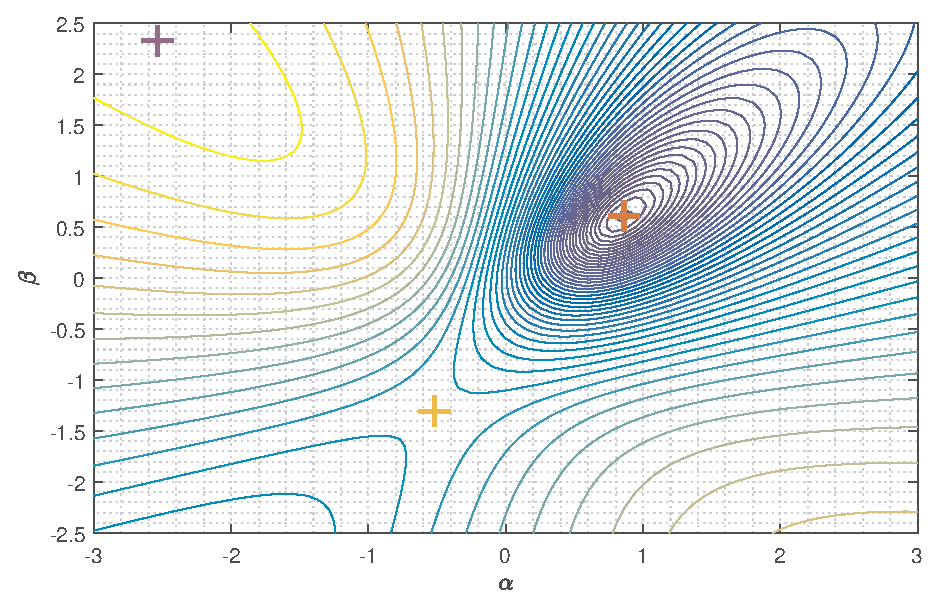
\includegraphics[width=\linewidth]{img/contour_f}
	\caption{Controur plot of the Raileight quotient in case of free damping, with stationary points}
	\label{fig:contour_f}
\end{figure}
\begin{figure}[H]
	\centering
	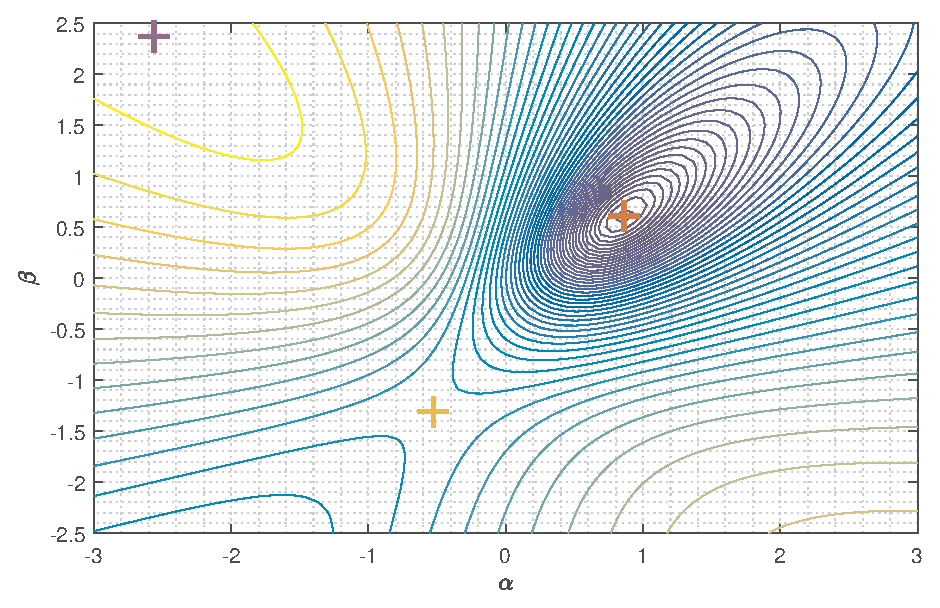
\includegraphics[width=\linewidth]{img/contour_p}
	\caption{Controur plot of the Raileight quotient in case of proportional damping, with stationary points}
	\label{fig:contour_p}
\end{figure}

	
\end{itemize}
	
%	 The first stationary point it's easy to find, but the other two are not. In order to find the other stationary points, the property of orthogonality of the modal shapes vector is used. The basic idea is to reduce a degree of freedom every frequency using this property. The procedure is the following:
%	\begin{itemize}
%		\item Provide an initial guess, the convergence to the first minima is quite robust to the first guess. Vector $[\ 1 \ 1 \ 1 \ ]\tr$ is used.
%		\item Use Matlab function \texttt{fminunc} to find the minima and the value of $x$, varying only two parameters of the vector ($x = [\ 1 \ \alpha \  \beta\ ]\tr$) 
%		\item Check if the minimum is the lowest frequency with a contour plot or performing the next steps. Define the first modal shape vector $u_{1R}$.  
%		\item Compute the null space of the first modal shape vector $Ker(u_{1R}\tr) $
%		\item find the minimum of
%		\begin{equation}
%			R_{q2} = \dfrac{[ \ 1 \ \alpha \ ] B_k\tr \bm K B_k [ \ 1 \ \alpha \ ]\tr}{[ \ 1 \ \alpha \ ] B_k\tr \bm M B_k [ \ 1 \ \alpha \ ]\tr}
%		\label{eq:rq2}
%		\end{equation}
%		where $img(B_k) = Ker(u_{1R}\tr)$ is a base of the Kernel of the first modal shape vector, the value of the function is another resonance frequency.
%		\item The last modal shape vector and the last resonance frequency can be computed respectively as a base of the Kernel of the two other modal shape vectors and evaluating $R_q$ at the last modal shape vector.
%		\begin{equation}
%			u_{3R} \in Ker(\left [
%			\begin{array}{cc}
%			u_{1R} &  u_{2R}
%			\end{array} \right ]\tr)
%		\end{equation}
%	\end{itemize}
%The results are shown in Table \ref{tab:modalResults} and the contour plot of the Raileight coefficient is shown in Figure \ref{fig:Rcontour}

\subsection{Matrix Iteration Method}
	Another method to find the eigenpairs is the Matrix Iteration Method. This method, as the name suggest, is an iterative method.
	Define the dynamic matrix:
	\begin{equation}
	    \label{eq:d_matrix}
		\bm{D} = \bm{K^{-1}}\bm{M}
	\end{equation}
	The algorithm
	\begin{enumerate}
		\item Define the first matrix $\bm{D}$ from Equation \eqref{eq:d_matrix}.
		\item Define a first guess of the vector $x$.
		\item Premultiply times the matrix $D$ the vector $x$ obtaining a new vector $x^+$.
		\begin{equation}
			x^+ = \bm{D}x
		\end{equation}
		\item Normalize the vector $x$ on the forst element.
		\begin{equation}
			x^+ = \dfrac{x}{x(1)}
		\end{equation}
		\item Repeat steps 3. and 4. on the new $x$.
		\item Repeat steps 3. 4. 5. N times. The greater the number of iteration N the greater the accuracy. In this case N=15 is chosen since the computation is not heavy.
		\item After the N iterations, the vector x converge to the first eigenvector of $\bm{D}$, the one with the highest eigenvalue (lowest frequency of the undamped system).
		\item The frequency is computed according to equation \eqref{eq:eig_mim}, the values of the frequency and the eigenvector are stored. The frequency is the square root of the reciprocal of the eigenvalue. The modal shape vectors are the eigenvectors (see comment \ref{com:eig_mim})
		\begin{equation}
		\label{eq:eig_mim}
		\begin{sistema}
			\omega_i = \left (\dfrac{x\tr D_i x}{x\tr x}\right )^{-\dfrac{1}{2}}\\
			u_i = x
		\end{sistema}
		\end{equation}
		\\ \\
	\noindent\textbf{ Matrix deflation}:
	Since the method can detect only the first eigenvector, to find the ther ones somehow an elimination of the first eigenvalue from the image of the matrix has to be performed. A manipulation can be used to achieve this effect: the matrix deflation. This procedure update the Matrix $D$ without affecting the eigenvectors, but reducing to zero a chosen eigenvalue. (Numerically it means reduce it to small values like $10^{-18}$)
		\item The matrix $D$ is updated performing the matrix deflation with the last eigenvalue.
		\begin{equation}
			\bm{D^+} =\bm{ D} - \dfrac{u_i u_i\tr \bm{M}}{u_i\tr \bm{M} u_i}
		\end{equation}
	\item The procedure from steps 3 to 9 is repeated for each additional eigenpair to find.
		
 \begin{comment}
 \label{com:eig_mim}
 	Equation \eqref{eq:eig_mim} comes from the standard eigenvalue problem in Box \ref{box:eig_prob}:
 	\begin{equation}
 	\label{eq:comment_eig_mim}
 	\left ( \bm{K}+\omega^2\bm{M}\right )x = 0 \Leftrightarrow \dfrac{x}{\omega^2} = \bm{K^{-1}}\bm{M}x \Leftrightarrow \dfrac{x}{\omega^2} = \bm{D}x
 	\end{equation}
 	From Equations \eqref{eq:comment_eig_mim} is evident that the eigenvalues of $\bm{D}$ are the reciprocals of the frequencies squared and the eigenvectors are the same as the modal shape vectors.
 \end{comment}
	\end{enumerate}
The whole procedure is performed for the case of free damping and the case of proportional damping. The results are shown in table \ref{tab:mim_results}.
	A block diagram which resumes the implemented method is shown in Figure \ref{fig:mim}. Again a orthogonality check is performed on the modal shape vectors.
	
	
	
	\begin{figure}[H]
		\centering
		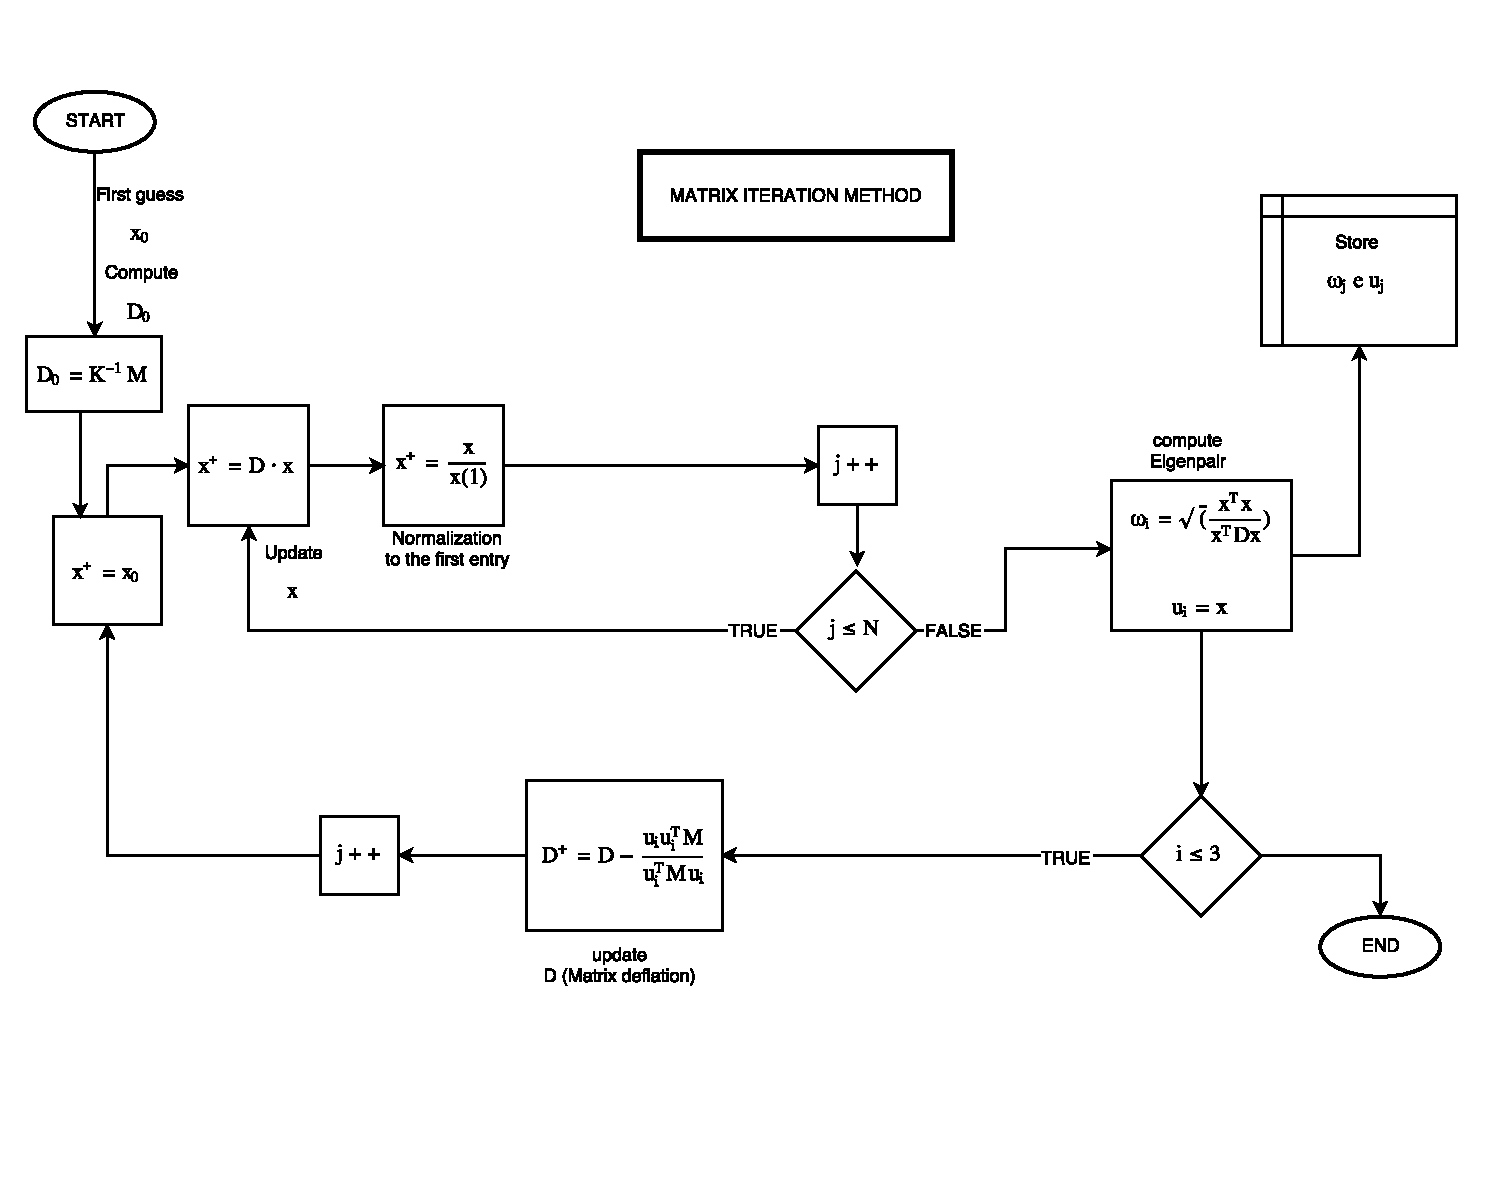
\includegraphics[width=\linewidth]{img/mim}
		\caption{the Matrix Iteration Method}
		\label{fig:mim}
	\end{figure}
	
\begin{table}[H]
	\centering
	\caption{Values of frequencies and modal shapes vector obtained using the Matrix Iteration Method}
	\label{tab:mim_results}
	\begin{tabular}{|l|lll|lll|}
		\hline
		& \multicolumn{3}{l|}{Free damping}                                                           & \multicolumn{3}{l|}{proportional damping}                                                   \\ \hline
		$\omega$  [rad/s]               & \multicolumn{1}{l|}{\rs{wm_f_1}} & \multicolumn{1}{l|}{\rs{wm_f_2}} & \rs{wm_f_3}  & \multicolumn{1}{l|}{\rs{wm_p_1}} & \multicolumn{1}{l|}{\rs{wm_p_2}} & \rs{wm_p_3}  \\ \hline
		\multirow{3}{*}{$\bm U$} & \rs{U_f_11}                     & \rs{Um_f_12}                     & \rs{Um_f_13} & \rs{Um_p_11}                     & \rs{Um_p_12}                     & \rs{Um_p_13} \\
		& \rs{Um_f_21}                     & \rs{Um_f_22}                     & \rs{Um_f_23} & \rs{Um_p_21}                     & \rs{Um_p_22}                     & \rs{Um_p_23} \\
		& \rs{Um_f_31}                     & \rs{Um_f_32}                     & \rs{Um_f_33} & \rs{Um_p_31}                     & \rs{Um_p_32}                     & \rs{Um_p_33} \\ \hline
	\end{tabular}
\end{table}


\subsubsection{Modal decomposition}
In the proportional damping case only the modal decomposition can be performed. Using the modal shape matrix $U$, definittively the one from the proprtional damping parameters. The new coordinates are:
\begin{subequations}
	\label{eq:modal_transf}
\begin{equation}
\label{eq:modal_coo}
	\tilde{x} = \bm{U\tr} x 
\end{equation}
The matrices becomes diagonal and they can be computed as shown below:
\par
\begin{tabularx}{\linewidth}{ X  X  X }
	\begin{equation}
		\bm{\tilde{M}} = \bm{ U\tr M U }
	\end{equation} &
	\begin{equation}
		\bm{\tilde{K}} = \bm{ U\tr K U }
	\end{equation} &
	\begin{equation}
		\bm{\tilde{C}} = \bm{ U\tr C U }
	\end{equation}
\end{tabularx}

\end{subequations}
\begin{comment}
In Equation \eqref{eq:modal_coo} it is possible to use the inverse of $U$ instead of the transpose to get the coordinates. This is due to the orthogonality property of $U$.\\
\end{comment}
The matrices are shown below.
 \begin{equation}
  \bm{\tilde{M}} = \input{result/M_s_matrix_tex.txt}
 \end{equation}
\begin{subequations}
\begin{equation}
	\tilde{\bm{K}} =  \left [ \ \tilde{K_1} \ \tilde{K_2} \ \tilde{K_3} \ \right ]
\end{equation}
\begin{equation}
	\tilde{K_1} =	\input{result/K_s_matrix_tex1.txt}
\end{equation}
\begin{equation}
	\tilde{K_2} =	\input{result/K_s_matrix_tex2.txt}
\end{equation}
\begin{equation}
	\tilde{K_3} =	\input{result/K_s_matrix_tex3.txt}
\end{equation}
\end{subequations}
\begin{equation}
\label{eq:C_modal}
	\bm{\tilde{C}} = c_a\bm{\tilde{M}} + c_b\bm{\tilde{K}} 
\end{equation}
\begin{comment}
Equation \eqref{eq:C_modal} comes from the fact that $c_b$ and $c_a$ are scalars.
\end{comment}

This decomposition uncouples the degree of freedom. It means each row of the matrix equation:
\begin{equation}
\bm{\tilde{M}} \ddot{\tilde{x}} + \bm{\tilde{C}} \dot{\tilde{x}} + \bm{\tilde{K}} \tilde{x} = \bm b
\label{eq:eqm:modal}
\end{equation}
can be treated as a single degree of freedom system.

\section{Transfer functions plots}
The transfer functions are converted from the state space form (Equation \eqref{eq:ss}) through the formula \eqref{eq:ss2tf}. The input is the voltage $v$.
\begin{equation}
\label{eq:ss2tf}
	\dfrac{X(s)}{V(s)} = C(sI-A)^{-1}B.
\end{equation}
To compute the transfer function between the force and the positions, the voltage-to-foce coefficient gain has to be removed. Given $F(s)$ the Laplace transform of the force signal.
\begin{equation}
	\dfrac{X(s)}{F(s)} = \dfrac{1}{g_v}\dfrac{X(s)}{V(s)}.
\end{equation}
The transfer function is a column vector with 3 entries, one for each output, they have the same denominator. The bode diagram are shown in Figure \ref{fig:bode_fp}. Both the cases are plotted: the free damping and and the proportional damping case. \\
\par \noindent
The two transfer function are barely distinguishable. The resonance peaks are clearly visible (different from the ones of the undamped version of the system).
%TODO very nice if you plot the comppsite TF and you find the natural frequencies!!!!
%TODO natural frequencies!!!!!!! 
\begin{figure}[H]
	\centering
	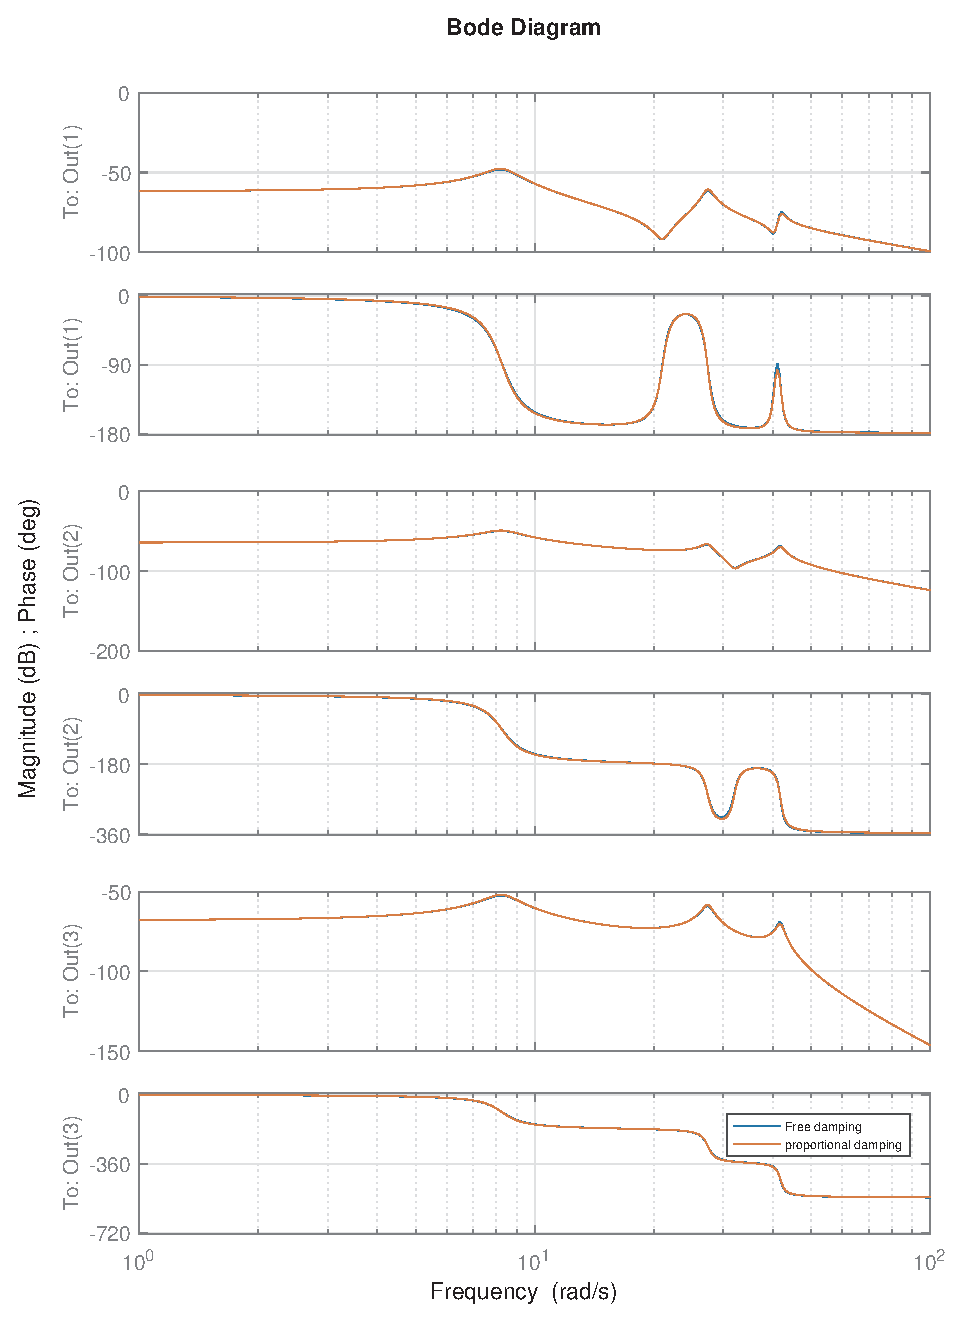
\includegraphics[width=\linewidth]{img/bode_fp}
	\caption{Bode diagram of the tranfer functions $\dfrac{X(s)}{F(s)}$}
	\label{fig:bode_fp}
\end{figure}

\section{Sine sweep analysis}
The inputs provided are two sine sweep signal with different sample frequencies. $5 ms$ and $10 ms$. The signal is the same, the only different is the sampling frequency.
To visualize the spectra of the signals, the fft is performed on both the signal. The spectrum is plotted with the real frequencies in \ref{fig:sinesweepspectra}.
\begin{figure}[H]
	\centering
	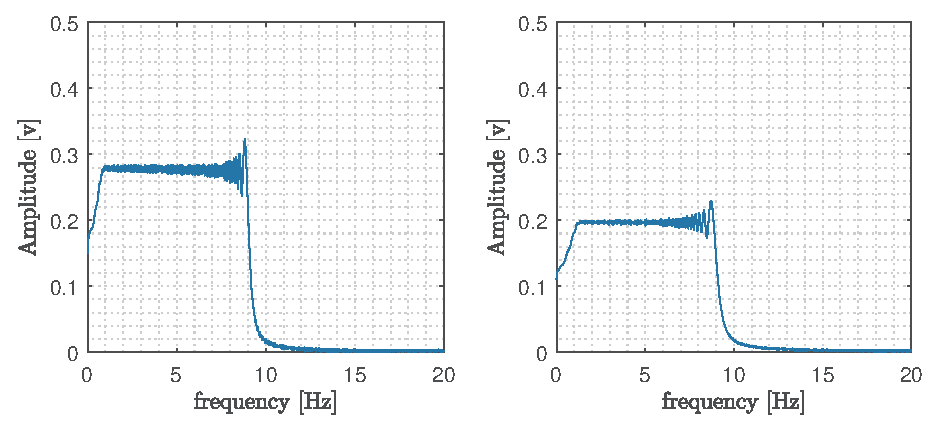
\includegraphics[width=\linewidth]{img/sine_sweep_spectra}
	\caption{Sine sweep spectra, (slow on the left and fast on the right)}
	\label{fig:sinesweepspectra}
\end{figure}
\noindent The two signal has the same frequency content. The difference is only the sampling time. The spectra cover all the resonance peaks of the transfer function. Despite the spectrum, the sine sweep excites each frequency for a limited amount of time (in fact a spectrogram is a more specific tool for the varying-in-time spectrum). From the time plot \ref{fig:sinesweeptime}, it is possible to notice that the third mode is not clearly visible .
\begin{figure}[H]
	\centering
	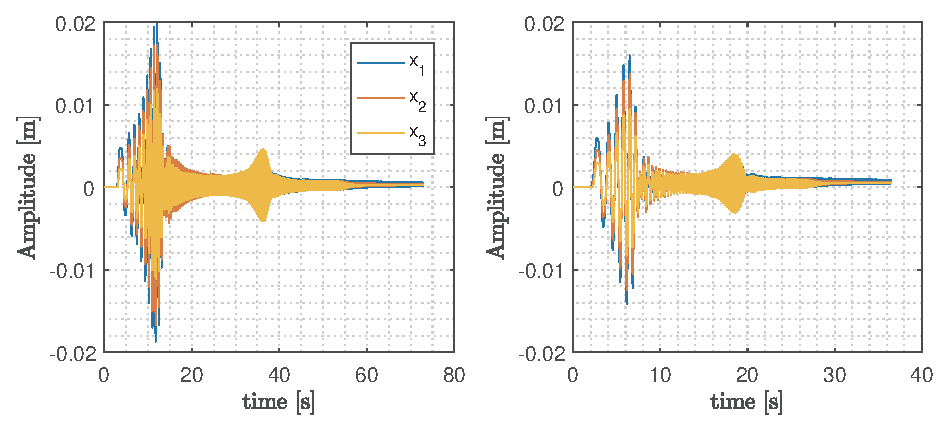
\includegraphics[width=\linewidth]{img/sine_sweep_time}
	\caption{Sine sweep outputs of the system, (slow on the left and fast on the right)}
	\label{fig:sinesweeptime}
\end{figure}
To estimate the transfer function from this data MATLAB provides several solution, the chosen one is
\texttt{tfest}. It is oriented to LSQ instead of some other method like \texttt{tfestimate}  which use the averaged periodogram method, and the signal is not periodic.
\begin{figure}[H]
	\centering
	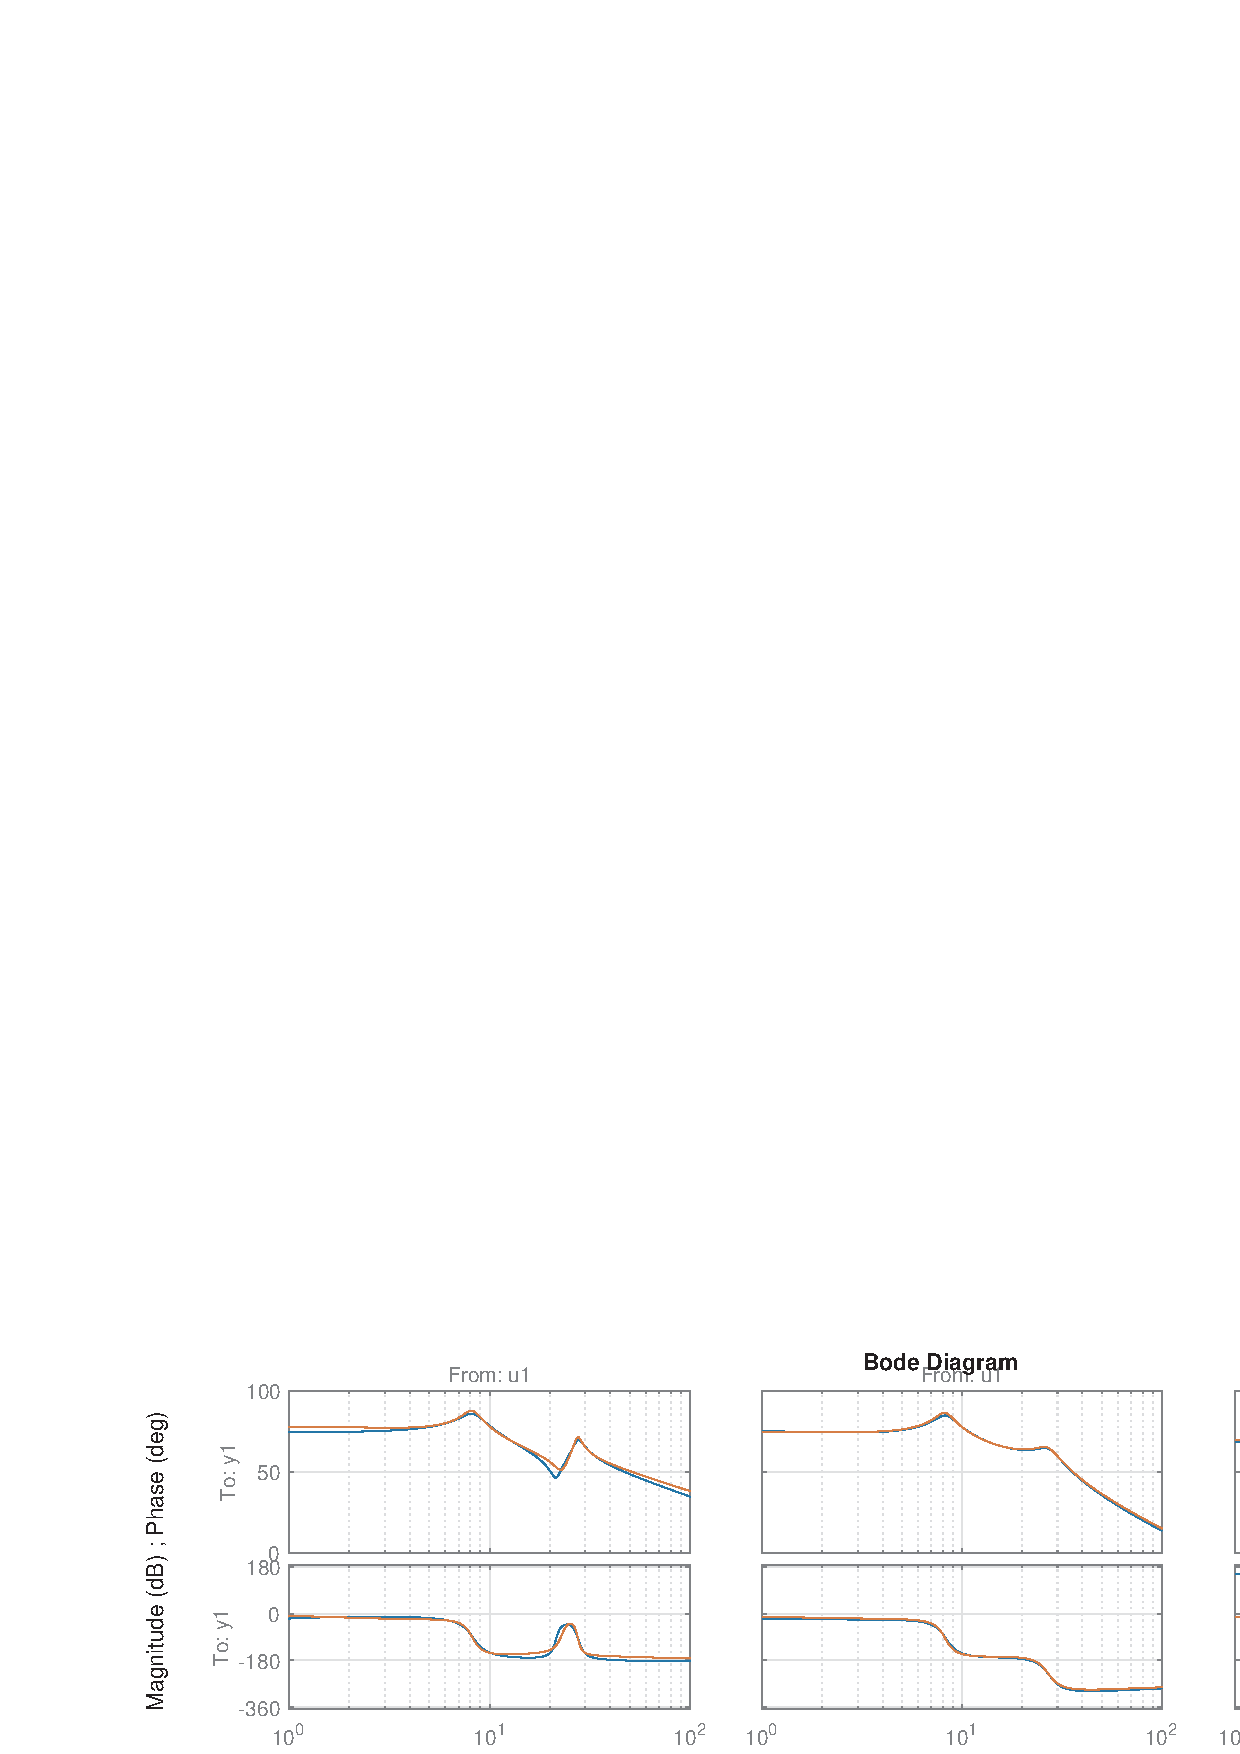
\includegraphics[width=\linewidth]{img/ssbode1}
	\caption{Sine sweep outputs of the system, (slow on the left and fast on the right)}
	\label{fig:ssbode1}
\end{figure}

%TODO CALCOLA FREQUENZE NATURALI E SMORZI

%TODO spiega proportional damping

%TODO trova gli smorzamenti modali, almeno spiegali

%TODO study the deflation matrix especially why the M matrix!!!

%TODO metti la normalizzazione dei modi perfavore OVUNQUE

%TODO scrivi che c'è un offset a steady state e lo si vede anche in g_v ogni volta diverso. Colpa attrito secco

%TODO metti in simulink lo state space con attrito (chiudi loop ed aggiungi a B la possibilità di attrito)

%TODO studia che succede in mult dof viscosi alle freq naturali

%TODO tabella al 
%TODO AGGIUNGI (t) alle variabili e lista dei simboli!
%TODO experimental set up
\end{document}